%UNIT 8: THE EFFECT OF VARYING A PARAMETER IN AUTONOMOUS DIFFERENTIAL EQUATIONS
%%%%%%%%%%%%%%%%%%%%%%%%%%%
%%%% Put the following at the top of each .tex file  %
\pagestyle{fancy}
\renewcommand{\theUnit}{8}
\ifthenelse{\isundefined{\UnitPageNumbers}}{}{\setcounter{page}{1}}
\rhead{Unit \theUnit: The Effect of Varying a Parameter in Autonomous Differential Equations}
\lhead{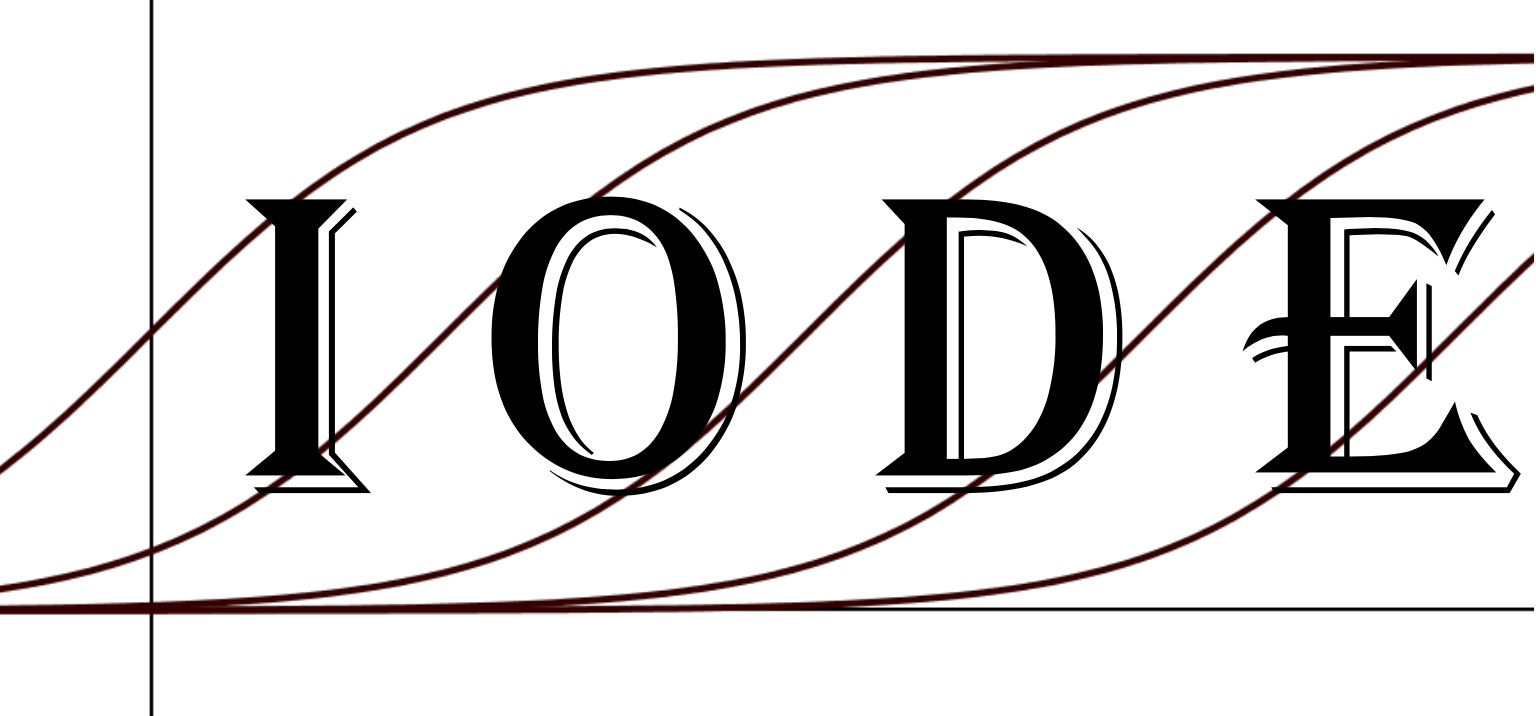
\includegraphics[width=1.25cm]{IODE-logo.png}}
\rfoot{\mypage}
\lfoot{}
\cfoot{}
\fancypagestyle{firstfooter}{\footskip = 50pt}
\renewcommand{\footrulewidth}{.4pt}
%%%%%%%%%%%%%%%%%%%%%%%%%%%
\vspace*{-20pt} \thispagestyle{firstfooter}
\pagebegin{Fish Harvesting}

A mathematician at a fish hatchery has been using the differential equation $\displaystyle\frac{dP}{dt}=2P\left(1-\frac{P}{25}\right)$ as a model for predicting the number of fish that a hatchery can expect to find in their pond.

\begin{enumerate}
\item Use an autonomous derivative graph, a phase line, and a slope field to analyze what this differential equation predicts for future fish populations for a range of initial conditions. Present all three of these representations and describe in a few sentences how to interpret them. \label{08problem1}
\clearpage

\item	Recently, the hatchery was bought out by fish.net and the new owners are planning to allow the public to catch fish at the hatchery (for a fee of course). This means that the previous differential equation used to predict future fish populations needs to be modified to reflect this new plan. For the sake of simplicity, assume that this new plan can be taken into consideration by including a constant, annual harvesting rate $k$ into the previous differential equation. Below are two modifications to the differential equation that may account for the new plan, as well as an option to create your own modification. Do you agree with (a) or (b)? If yes, explain why. If no, create your own modification and explain your reasoning. \label{08problem2} \\
\vs
\begin{enumerate*} 
\item $\displaystyle \frac{dP}{dt}=2P\left(1-\frac{P}{25}\right)-kP$ \hspace{.5in}
\item $\displaystyle \frac{dP}{dt}=2P\left(1-\frac{P-k}{25}\right)$ \hspace{.5in}
\item Create Your Own
\end{enumerate*}
\clearpage
	
\item	Your team of consultants settled on $\displaystyle\frac{dP}{dt} = 2P\left(1-\frac{P}{25}\right) - k$ to model the new fishing plan.  Analyze the effect of different choices for the value of k on the fish population. Synthesize your analysis in a \textbf{one page} report for the new owners that illustrates the implications that various choices of $k$ will have on future fish populations. Your report may include one or more graphical representations but must communicate the effect of different $k$ values in a concise way. \label{08problem3}

\clearpage

\item In studying climate, scientists are often concerned about positive feedback loops: two or more processes that amplify each other, creating a system of amplification that leads to a vicious cycle. One example is the interaction of water vapor with global temperature. If global temperature increases, the capacity of the atmosphere to contain evaporated water vapor also increases. If water resources are available, this would result in an increased amount of water vapor in the atmosphere. Water vapor is a greenhouse gas, thus if a climate system has more water vapor in the atmosphere, the global temperature will increase due to the increased insulation of the atmosphere. This positive feedback loop will eventually equilibrate at a higher temperature. Some scientists predict that a global increase in average temperature of just two degrees would be enough to kick off a system of positive feedback loops that would equilibrate at a temperature at least 6 degrees higher than we have now. This 6-degree increase would be enough to turn rainforests into deserts and melt ice caps. It may even redistribute the areas of the world that can support human life, i.e. making previously uninhabitable places, like the northern reaches of Siberia and Canada, inhabitable (though they may not support agriculture) and previously inhabitable places, like coastal cities, uninhabitable. \label{08problem4}

\begin{enumerate}
\item A modern pre-industrial average temperature at the equator is about 20 degrees Celsius. Assuming that our current global climate system has not undergone this vicious cycle, model this system with a phase line. What are the essential features of that phase line? \label{08problem4parta}
\vfill
\item What is a simple differential equation that corresponds to your above phase line? \label{08problem4partb}
\vfill
\clearpage
\item A group of scientists came up with the following model for this global climate system:
\[
\frac{dC}{dt} = \frac{1}{10}\Big(C-20\Big)\Big(22-C\Big)\Big(C-26\Big)-k
\]
where $C$ is the temperature, in Celsius, and $k$ is a parameter that represents governmental regulation of greenhouse gas emissions. Assume the baseline regulation corresponds to $k=0$, increasing regulation corresponds to increasing $k$, and the current equatorial temperature is around 20 degrees. To what equatorial temperature will the global climate equilibrate? \label{08problem4partc}
\vfill
\item Sketch a bifurcation diagram and use it to describe what happens to the global temperature for various values of $k$. \label{08problem4partd}
\vfill
\clearpage
\item Suppose at the start of a new governmental administration, the temperature at the equator is about 20 degrees Celsius, and $k=0$. Based on the model and other economic concerns, a government decides to deregulate emissions so that $k=-0.5$. Later, the Smokestack Association successfully lobbied for a 5\% change, resulting in $k=-0.525$. Subsequently, a new administration undid that change, reverting to $k=-0.5$, and eventually back to $k=0$. What is the equilibrium temperature at the equator after all of these changes? \label{08problem4parte}
\clearpage
\item Use your bifurcation diagram to propose a plan that will return the temperature at the equator to 20 degrees Celsius. \label{08problem4partf} \vfill

\end{enumerate}

\end{enumerate}
\clearpage
\pagebegin{Homework Set 8}

\begin{enumerate}
\item
\begin{enumerate}
\item The owners of fish.net have settled on model $dP/dt = 2 P (1-P/25) - k$ to make their business decisions, where $P$ is the number of fish in thousands, and $k$ is a harvesting rate measured in thousands of fish per year. They initially allow a harvesting rate $k = 12$. If they allow fishing to continue for a while at this rate, what does their model predict for the long term number of fish in the lake? \label{08HWproblem1parta}
\item The early years of fish harvesting went well, so they increased the harvesting rate by a modest amount.  They now allow harvesting rate corresponding to $k = 13$.  What does this model predict will be the long term result of this fishing practice? \label{08HWproblem1partb}
\item The owners of fish.net panicked when their fish population reached $P=5$ and decided to return to their original business model with $k=12$.  Will the fish population return to the levels you described in problem \ref{08HWproblem1parta}?  Why or why not? \label{08HWproblem1partc}
\end{enumerate}

\item The bifurcation diagram for an autonomous differential equation $dy/dt = f(y)$ is shown below.  The solid parts corresponds to stable equilibria and the dashed part is for unstable ones.  $f(y)$ has a parameter $c$, and changing the value of that parameter changes the behavior of the system, as shown.  \label{08HWproblem2} \\
\begin{center}
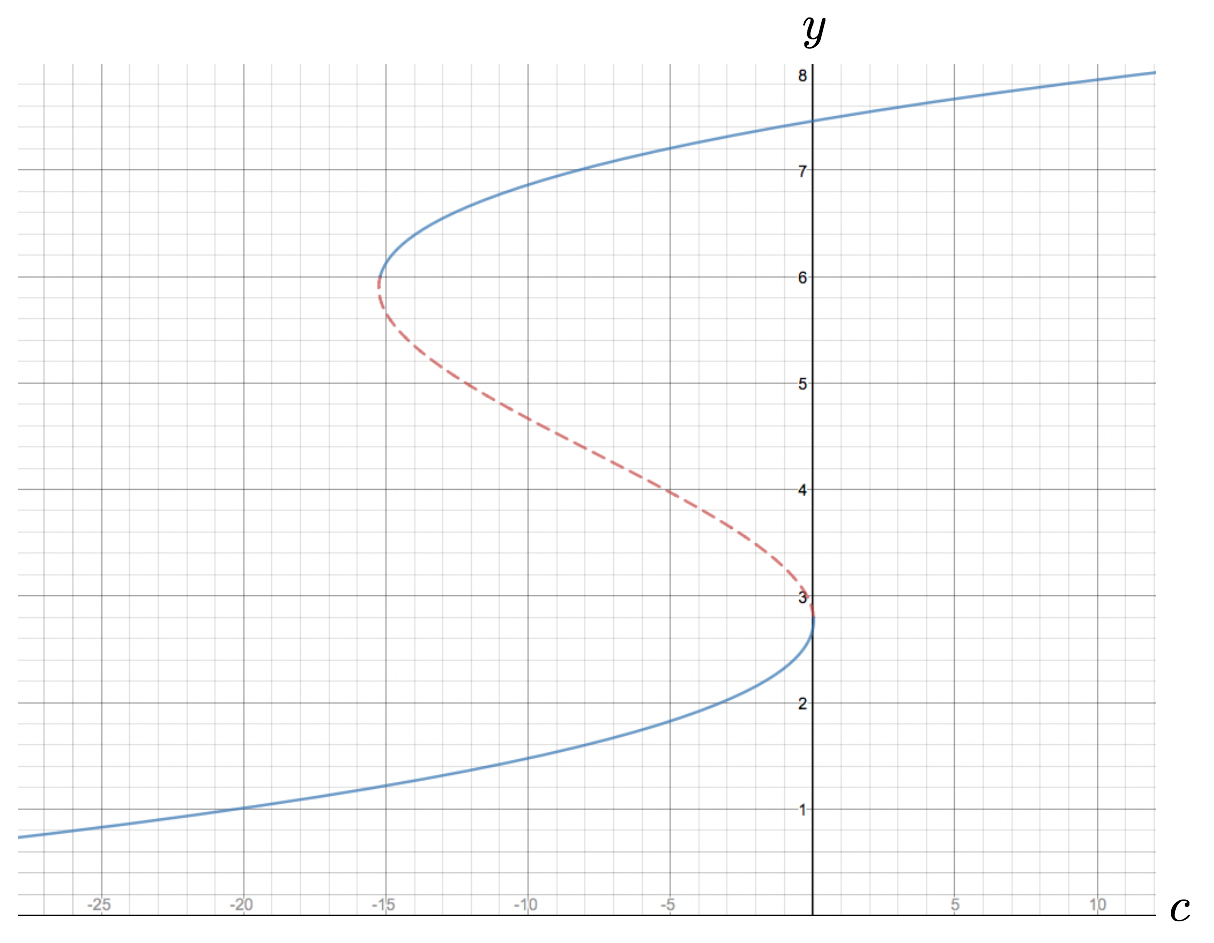
\includegraphics[width=5in]{08/08Bifurcation.png}
\end{center}
\clearpage
\begin{enumerate}
\item Sketch the phase lines when $c=-20$, $c=-5$, $c=0$, and $c=10$. \label{08HWproblem2parta}
\item Sketch the corresponding graphs of $y$ vs. $t$ for each of the choices of $c$ listed above. \label{08HWproblem2partb}
\item For what values of $c$ does the system have two attractors? \label{08HWproblem2partc}
\item As shown, the bifurcation diagram has two stable (solid) ``branches'' connected by an unstable (dashed) branch. Would it be possible for the entire curve to be stable? Why or why not?	 \label{08HWproblem2partd}
\item If this model represents a physical system, and you measure that the system has a steady state of $y = 2$, what value of $c$ should you choose for your model? \label{08HWproblem2parte}
\item Again, let's think of this model as representing some physical system, similar to the hatchery example we considered in class. You are the owner of that system, and you have control over the value of $c$. $y(t)$ represents the state of your system at a given time. Consider the following experiment. \label{08HWproblem2partf}
\begin{enumerate}
\item Let's say the system starts with an initial condition of $y(0) = 0$, and you fixed $c$ at $c = -10$. After a long time elapses, what value does $y$ approach? \label{08HWproblem2partfi}
\item Assume that $y$ has evolved to your answer in problem \ref{08HWproblem2partfi}, and that result is not something you are completely happy with. You've heard that a company down the road is using $c = 10$, so you make that change. What value does $y$ approach now (after substantial time has passed)? \label{08HWproblem2partfii}
\item Assume that $y$ has evolved now to your answer in \ref{08HWproblem2partfii}. Unfortunately, this new value of $y$ is even worse than the old one, so you want to change $c$ back to $c = -10$. Will the system evolve back to your answer in problem \ref{08HWproblem2partfi}? Explain. \label{08HWproblem2partfiii}
\end{enumerate}
\end{enumerate}

\item For each of the following, illustrate with suitable solution function graphs and/or phase lines the way in which the solutions change as the value of $r$ changes. Identify the precise value(s) of $r$ for which there is a either a change in the number of equilibrium solution(s) or a change in the type of equilibrium solution(s). Explain in words the change that happens at each significant value of $r$ identified. 

\begin{enumerate}
\item $\displaystyle \frac{dy}{dt}=(y-3)^2+r$ \label{08HWproblem3parta}
\item $\displaystyle \frac{dy}{dt}=y^2-ry+1$ \label{08HWproblem3partb}
\item $\displaystyle \frac{dy}{dt}=ry+y^3$ \label{08HWproblem3partc}
\item $\displaystyle \frac{dy}{dt}=y^6-2y^4+r$ \label{08HWproblem3partd}
\end{enumerate}

\item For problem \ref{08HWproblem3parta}, sketch a graph of the equilibrium solutions as $r$ varies. Such a graph is referred to as ``bifurcation diagram'' and the significant values of $r$ are called ``bifurcation values.'' \label{08HWproblem4}
\item For problem \ref{08HWproblem3partb}, sketch a bifurcation diagram and identify the bifurcation values. \label{08HWproblem5}
\item For problem \ref{08HWproblem3partc}, sketch a bifurcation diagram and identify the bifurcation values. Why might this bifurcation be called a ``pitchfork bifurcation?'' \label{08HWproblem6}
\end{enumerate}



